\documentclass{cours}

\title{Géométrie Vectorielle dans l'Espace}

\begin{document}
    \maketitle{8}

    \begin{Gpartie}{Vecteurs de l'Espace} 
        La notion de vecteur se généralise à l'espace.

        Le vecteur $\vec{u}$ est caractérisé par un sens, une direction, et une norme, notée $\lvert\lvert{\vec{u}}\rvert\rvert$.
        \begin{Spartie}{Théorème} 
            $A$, $B$, et $C$ étant quatre points de l'espace, les propositions suivantes sont équivalentes :
            \begin{itemize}
                \item $\overrightarrow{AB}=\overrightarrow{CD}$
                \item Le quadrilatère $ABCD$ est un parallélogramme.
                \item Les segments $\big[AD\big]$ et $\big[BC\big]$ ont le même milieu.
            \end{itemize}
        \end{Spartie}
        \begin{Spartie}{Définition} 
            Deux vecteurs de l'espace $\vec{u}$ et $\vec{v}$ sont \emph{colinéaires} si et seulement si il existe un réel $k$ tel que $\vec{u}=k\vec{v}$ ou $\vec{v}=k\vec{u}$.
        \end{Spartie}
        \begin{Spartie}{Propriété} 
            Toutes les opérations sur les vecteurs, en particulier la relation de Chasles sont identiques dans l'espace comme dans le plan.
        \end{Spartie}
        \begin{Spartie}{Theorème} 
            $A$ et $B$ étant deux points distincts de l'espace, $\big(AB\big)$ est l'ensemble des points $M$ de l'espace tels que $\overrightarrow{AM}=t \overrightarrow{AB},\ t\in\mathbb{R}$

            $\big(AB\big)=\big\{~M\in\mathcal{E},~\overrightarrow{AM}=t\overrightarrow{AB},~t\in\mathbb{R}~\big\}$
        \end{Spartie}
        \begin{Spartie}{Définition} 
            Un vecteur $\vec{k}$ est une \emph{combinaison linéaire} des vecteurs $\vec{u}$, $\vec{v}$ et $\vec{w}$ s'il existe des réels $a$, $b$ et $c$ tels que $\vec{k}=a\vec{u}+b\vec{v}+c\vec{w}$
        \end{Spartie}
    \end{Gpartie}
    \begin{Gpartie}{Vecteurs Coplanaires} 
        \begin{Spartie}{Définition} 
            Des vecteurs sont \emph{coplanaires} s'ils admettent des représentants dont les extrémités sont dans un même plan.
            \begin{center}
                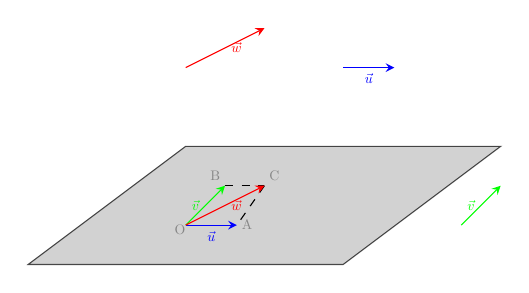
\begin{tikzpicture}
                    \coordinate (O) at (-1,0) {}; \draw (O) node[anchor=north east, scale=0.5, inner sep=0pt] {O};
                    \coordinate (A) at (-0.35,0) {}; \draw (A) node[anchor=west, scale=0.5] {A};
                    \coordinate (B) at (-0.5,0.5) {}; \draw (B) node[anchor=south east, scale=0.5] {B};
                    \coordinate (C) at (0,0.5) {}; \draw (C) node[anchor=south west, scale=0.5] {C};
                    \draw[fill=lightgray, opacity=0.7] (-3,-0.5) -- (1,-0.5) -- (3,1) -- (-1,1) -- cycle;
                    \draw[dashed] (B) -- (C);
                    \draw[dashed] (C) -- (A);
                    \draw[-stealth, blue] (O) -- (A) node [midway, label={[scale=0.5, label distance=-6pt]below:$\vec{u}$}] {};
                    \draw[-stealth, green] (O) -- (B) node [midway, label={[scale=0.5, label distance=-6pt]left:$\vec{v}$}] {};
                    \draw[-stealth, red] (O) -- (C) node [midway, label={[scale=0.5, label distance=-6pt]right:$\vec{w}$}] {};

                    \draw[-stealth, blue] (1,2) -- (1.65,2) node [midway, label={[scale=0.5, label distance=-6pt]below:$\vec{u}$}] {};
                    \draw[-stealth, green] (2.5,0) -- (3,0.5) node [midway, label={[scale=0.5, label distance=-6pt]left:$\vec{v}$}] {};
                    \draw[-stealth, red] (-1,2) -- (0,2.5) node [midway, label={[scale=0.5, label distance=-6pt]right:$\vec{w}$}] {};
                \end{tikzpicture}
                \parbox{\linewidth}{\captionof{figure}{Illustration de la Définition}}
            \end{center}
            Si $O$ est un point quelconque et $A$, $B$ et $C$ sont tels que $\overrightarrow{OA}=\vec{u},\ \overrightarrow{OB}=\vec{v},\ \text{et}\ \overrightarrow{OC}=\vec{w}$

            $\vec{u}$, $\vec{v}$, et $\vec{s}$ coplanaires $\iff$ $O$, $A$, $B$, et $C$ coplanaires
        \end{Spartie}
        \begin{Spartie}{Théorème} 
            $\vec{u}$, $\vec{v}$ et $\vec{w}$ étant trois vecteurs de l'espace avec $\vec{u}$ et $\vec{v}$ non colinéaires.

            $\vec{u}$, $\vec{v}$ et $\vec{w}$ sont coplanaires si et seulement si il existe deux réels $\alpha$ et $\beta$ tels que $\vec{w}=\alpha\vec{u}+\beta\vec{v}$. \quad\big($\vec{w}$ est une \emph{combinaison linéaire} de $\vec{u}$ et $\vec{v}$\big)
            \begin{SSpartie}{Démonstration} 
                Soient $O$, $A$, $B$, et $C$ quatre points tels que $\overrightarrow{OA}=\vec{u},~\overrightarrow{OB}=\vec{v}$ et $\overrightarrow{OC}=\vec{w}$

                $\vec{u}$ et $\vec{v}$ sont non-colinéaires donc, $O$, $A$ et $B$ sont non alignés, et $\big(OAB\big)$ est un plan de base $\left(O\,,\overrightarrow{OA}\,,\overrightarrow{OB}\right)$
                \begin{itemize}[leftmargin=7ex]
                    \item[``$\implies$''] On suppose que $\vec{u}$, $\vec{v}$, et $\vec{w}$ sont coplanaires. Alors, $C\in\big(OAB\big)$. \\ $C$ admet donc des coordonnées $\big(\alpha\,;\beta\big)$ dans la base $\left(O\,,\overrightarrow{OA}\,,\overrightarrow{OB}\right)$. C'est-à-dire $\overrightarrow{OC}=\alpha\overrightarrow{OA}+\beta\overrightarrow{OB}$ ou encore $\vec{w}=\alpha\vec{u}+\beta\vec{v}$.$\quad\square$
                    \item[``$\impliedby$''] On suppose que $\vec{w}=\alpha\vec{u}+\beta\vec{v}$ \\ Soit $D$ le point de $\big(OAB\big)$ de coordonnées $\big(\alpha\,;\beta\big)$ \\ Alors, 
                     
                    $\begin{aligned}[t]
                        \overrightarrow{OD}&=\alpha\overrightarrow{OA}+\beta\overrightarrow{OB} \\
                        &=\alpha\vec{u}+\beta\vec{v}=\vec{w}=\overrightarrow{OC}
                    \end{aligned}$

                    Donc, $D=C$, les points sont confondus, et comme $C\in\big(OAB\big)$, $\vec{u}$,~$\vec{v}$,~et~$\vec{w}$ sont coplanaires.$\quad\square$
                \end{itemize}
            \end{SSpartie}
            \begin{SSpartie}{Théorème : Caracterisation Vectorielle d'un Espace} 
                Si $A$, $B$, et $C$ sont trois points non-alignés de l'espace, le plan $\big(ABC\big)$ est l'ensemble des M tels que : \[\overrightarrow{AM}=t\overrightarrow{AB}+t'\overrightarrow{AC}\quad\big(~t,~t'\in\mathbb{R}~\big)\]
            \end{SSpartie}
        \end{Spartie}
    \end{Gpartie}
    \vspace{-0.7cm} % to get last line of vocabulaire to fit on page
    \begin{Gpartie}{Repèrage dans l'Espace} 
        \begin{Spartie}{Définition} 
            Un repère de l'espace est constitué d'un point appelé origine du repère (en général $O$) et d'un triplet de vecteurs non-coplanaires (en général $\vec{\imath}$, $\vec{\jmath}$ et $\vec{k}$)

            On le note $\left(O\,;\vec{\imath}\,,\vec{\jmath}\,,\vec{k}\right)$
        \end{Spartie}
        \begin{Spartie}{Vocabulaire} 
            La droite $\big(O\,;\vec{\imath}\big)$ est appelée axe des \emph{abscisses}.

            La droite $\big(O\,;\vec{\jmath}\big)$ est appelée axe des \emph{ordonnées}.

            La droite $\big(O\,;\vec{k}\big)$ est appelée axe des \emph{cotes}.

            Lorsque ces trois axes sont perpendiculaires deux à deux, le repère est \emph{orthogonal}. \\ Si de plus $\lvert\lvert\vec{\imath}\rvert\rvert=\lvert\lvert\vec{\jmath}\rvert\rvert=\lvert\lvert\vec{k}\rvert\rvert=1$, le repère est \emph{orthonormé}.
        \end{Spartie}
        \begin{Spartie}{Coordonnées dans l'Espace} 
            \begin{SSpartie}{Théorème} 
                Si $\left(O\,;\vec{\imath}\,,\vec{\jmath}\,,\vec{k}\right)$ est un repère, pour tout point $M$, il existe un unique triplet $\big(x\,; y\,; z\big)$ de réels tels que $\overrightarrow{OM}=x\vec{\imath}+y\vec{\jmath}+z\vec{k}$, appelés coordonnées de $M$.

                On note $M~\big(x\,;y\,;z\big)$
                \begin{SSSpartie}{Démonstration} 
                    % \begin{center}
                        % \begin{tikzpicture}
                            % \includegraphics[width=10cm]{example-image}
                            % \parbox{\linewidth}{\captionof{figure}{Démonstration du Théorème}}        
                        % \end{tikzpicture}
                    % \end{center}
                    $\overrightarrow{OM}=\overrightarrow{OM'}+\overrightarrow{M'M}$ \\
                    Or $M\in\left(O\,;\vec{\imath}\,;\vec{\jmath}\right)$ donc il a des coordonnées $\big(x\,; y\big)$ dans le~repère~$\left(O\,;\vec{\imath}\,;\vec{\jmath}\right)$.

                    $\overrightarrow{OM'}=x\vec{\imath}+y\vec{\jmath}$

                    $\overrightarrow{M'M}$ est colinéaire à $\vec{k}$ (on a projeté dans sa direction). Il existe un réel $z$ tek que $\overrightarrow{M'M}=z\vec{k}$

                    Donc, $\overrightarrow{OM}=x\vec{\imath}+y\vec{\jmath}+z\vec{k}\quad\square$ \\
                    (On admet l'unicité)
                \end{SSSpartie}
                \begin{SSSpartie}{Remarque} 
                    On définit de même les coordonnées d'un vecteur de l'espace. Tout vecteur de l'espace est une combinaison linéaire des vecteurs $\vec{\imath}$, $\vec{\jmath}$ et $\vec{k}$.
                \end{SSSpartie}
            \end{SSpartie}
            \begin{SSpartie}{Théorème} 
                Si dans un repère $A~\big(x_A\,; y_A\,; z_A\big)$ et $B~\big(x_B\,; y_B\,; z_B\big)$ sont deux points, le vecteur $\overrightarrow{AB}$ a pour coordonnées : 
                \[\overrightarrow{AB}~\begin{psmallmatrix} x_B-x_A \\ y_B-y_A \\ z_B-z_A \end{psmallmatrix}\]
                Et $I$, le point du milieu de $\big[AB\big]$ :
                \[I~\Bigg(~\frac{x_A+x_B}{2}~;~\frac{y_A+y_B}{2}~;~\frac{z_A+z_B}{2}~\Bigg)\]
                Dans un repère orthonormé, un vecteur $\vec{u}~\begin{psmallmatrix}x \\ y \\ z\end{psmallmatrix}$ a pour norme :
                \[\lvert\lvert\vec{u}\rvert\rvert=\sqrt{x^2+y^2+z^2}\]
                \begin{SSSpartie}{Démonstration} 
                    Passer par $M'$, le projeté orthogonal de $M$ sur $\left(O\,;\vec{\imath}\,,\vec{\jmath}\right)$, puis appliquer le théorème de Pythagore deux fois.
                \end{SSSpartie}
            \end{SSpartie}
            \begin{SSpartie}{Théorème} 
                Si $I$ est le milieu de $\big[AB\big]$, pour tout $M$ :
                \[\overrightarrow{MI}=\tfrac{1}{2}\overrightarrow{MA}+\tfrac{1}{2}\overrightarrow{MB}\]
                \begin{SSSpartie}{Démonstration} 
                    $\begin{aligned}[t]
                        \overrightarrow{MI}&=\overrightarrow{MA}+\overrightarrow{AI} \\
                        &=\tfrac{1}{2}\overrightarrow{MA}+\tfrac{1}{2}\overrightarrow{MA}+\tfrac{1}{2}\overrightarrow{AB} \\
                        &=\tfrac{1}{2}\overrightarrow{MA}+\tfrac{1}{2}\overrightarrow{MB}\quad\text{(Chasles)}
                    \end{aligned}$
                \end{SSSpartie}
            \end{SSpartie}
        \end{Spartie}
    \end{Gpartie}
\end{document}